\section{Decomposition 1: SIoTIP System (Av3, P2, UC11, UC14, UC15, UC18)}
\subsection{Module to decompose}
    In this run we decompose the \texttt{SIoTIP System}.

\subsection{Selected architectural drivers}
    The non-functional drivers for this decomposition are:
    \begin{itemize}
    	\item \emph{Av3}: Pluggable device or mote failure
    	\item \emph{P2}: Requests to the pluggable data database
    \end{itemize}

    \noindent The related functional drivers are:
    \begin{itemize}
        \item \emph{UC11}: Send pluggable device data (P2) \\
              This use case stores pluggable device data in the pluggable device data storage.
              This could be a sensor reading, or an actuator status.
    	\item \emph{UC14}: Send heartbeat (Av3) \\
              This use case checks whether or not motes and pluggable devices
              are still operational.
    	\item \emph{UC15}: Send notification (Av3) \\
              This use case sends a notification to a registered user.
    	\item \emph{UC18}: Check and deactivate applications (Av3) \\
              This use case deactivates any application that requires deactivation,
              because of unavailability of essential pluggable devices
              or unassigned mandatory roles.
    \end{itemize}

    \paragraph{Rationale}
    We chose Av3 first since it had high priority and it was more relevant to
    the core of the system (pluggable device data) than attributes M1 and U2. We
    chose P2 along with Av3 as it would force us to think about the way
    sensor data is handled. We believe this combination of pluggable device connectivity and
    storage of sensor data is the most defining feature of the system, and that
    handling this combination would give a better starting point than M1+U2
    for later ADD iterations.

\subsection{Architectural design}
    \paragraph{Application redundancy settings for Av3}
    Discussion of the solution selected for (a part of) one of the architectural
    drivers.

    \paragraph{Failure detection for Av3}
    timers? \\
    heartbeat/timestamp tactic

    \paragraph{Application deactivation for Av3}
    same as Application redundancy settings for Av3? \\
    degradation/removal from service tactic

    \paragraph{Notifications for Av3}
    from application manager to cust orgs and apps \\
    from gateway to infr owners \\
    notifications tactic

    \paragraph{Scheduling for P2}
    dynamic priority scheduling \\
    tactics: schedule resource, prioritize events, also limit event response?\\
    starvation avoidance \\
    \textit{TODO ASK: The  system  checks  whether  the  pluggable  device  
    has  been  initialised (cf. UC8: Initialise  a pluggable device)}

    \paragraph{Pluggable data separation for P2}
    "pluggable data has no impact on other data"
    two databases

\subsubsection{Alternatives considered}
    \paragraph{Alternatives for X}
    A discussion of the alternative solutions and why that were not selected.

\subsection{Instantiation and allocation of functionality}
    \paragraph{Decomposition}
    Main aspects of the resulting decomposition.

    \subparagraph{PluggableDeviceFacade}
    send heartbeats

    \subparagraph{GatewayFacade}
    receive heartbeats, send heartbeats/device lists, send application shutdown, send notification trigger (Av3)\\
    forward data to applications

    \subparagraph{HeartbeatProcessor}
    process heartbeats: check timers (Av3)

    \subparagraph{PluggableDeviceManager}
    check list of devices and see if there are pluggable devices for applications
    check redundancy in the available pluggable devices
    contains application preferences (e.g. amount of sensors required)
    can send command to deactivate application
    If failure detected, notify inf owner (Av3).
    reactivate application if new/needed hardware detected

    \subparagraph{RequestHandler}
    handles requests from gateways and sends them to other components
    handles requests from other components and sends them to gateways

    \subparagraph{ApplicationManager}
    deactivate apps
    ???? check mandatory user roles
    set redundancy in the available pluggable devices
    If application suspended or re-activated, notify cust. org.
    If application uses failed plugg device, notify application
    (Av3)

    \subparagraph{NotificationHandler}
    Send notifications. \\
    stored by system \(->\) contact DB? \\
    lookup communication channel \\
    users choose delivery method?

    \begin{figure}[!htp]
    	\centering
    	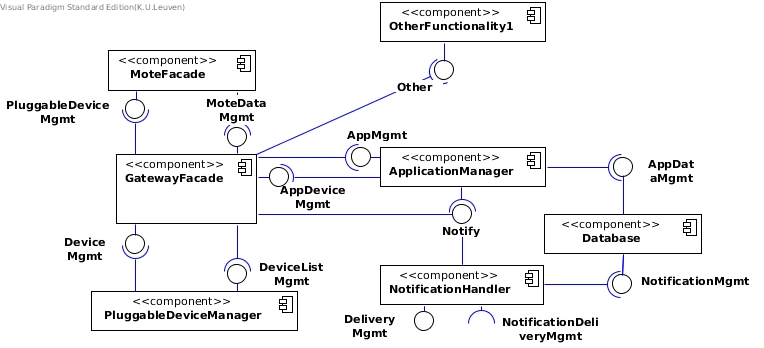
\includegraphics[width=0.8\textwidth]{component-diagram-1}
    	% \missingfigure[figwidth=0.8\textwidth]{Component-and-connector diagram}
    	\caption{Component-and-connector diagram of this decomposition.}
        \label{fig:it1-cc_main}
    \end{figure}

    \paragraph{Behaviour}
    If needed and explanation of the behaviour of certain aspects of the design so
    far.

    \begin{figure}[!htp]
    	\centering
    	%\includegraphics[width=0.8\textwidth]{}
    	\missingfigure[figwidth=0.8\textwidth]{Sequence diagram}
    	\caption{Sequence diagram illustrating a key behavioural aspect.
    	}\label{fig:it1-seq_aspect1}
    \end{figure}

    \paragraph{Deployment}
    Rationale of the allocation of components to physical nodes.

    \begin{figure}[!htp]
    	\centering
    	%\includegraphics[width=0.8\textwidth]{}
    	\missingfigure[figwidth=0.8\textwidth]{Deployment diagram}
    	\caption{Deployment diagram of this decomposition.
    	}\label{fig:it1-depl_main}
    \end{figure}

\subsection{Interfaces for child modules}
    \subsubsection{ModuleB}
    \begin{itemize}
    	\item InterfaceA
    	\begin{itemize}
    		\item \texttt{returnType operation1(ParamType param1)} throws TypeOfException
    		\begin{itemize}
    			\item Effect: Describe the effect of calling this operation.
    			\item Exceptions:
    			\begin{itemize}
    				\item TypeOfException: Describe when this exception is thrown.
    			\end{itemize}
    		\end{itemize}

    		\item \texttt{returnType operation2()}
    		\begin{itemize}
    			\item Effect: Describe the effect of calling this operation.
    			\item Exceptions: None
    		\end{itemize}
    	\end{itemize}
    \end{itemize}

\subsection{Data type definitions}
    Describe per complex data type used in the interfaces what it represents.

    \paragraph{returnType} This data element represents X.

    \paragraph{ParamType} This data element represents Y.

\subsection{Verify and refine}
    This section describes per component which (parts of) the remaining
    requirements it is responsible for.

    \paragraph{ModuleB}
    \begin{itemize}
    	\item \emph{Z1}: name
    	\item \emph{UCd}: name
    \end{itemize}

    \paragraph{ModuleC}
    \begin{itemize}
    	\item \emph{UCba}: name\\Description which part of the original use case is
    	the responsibility of this component.
    \end{itemize}
